\chapter{Traitement d'images 2}  

{\footnotesize
\begin{itemize}
\item Logiciel\footnote{Le logiciel Gimp est librement téléchargeable : \url{http://www.gimp.org/}} : \emph{Gimp}
\item Prérequis (se reporter si nécessaire aux \emph{Fiches MITIC 6\up{e}}) :
        \begin{itemize}
        \item recadrer une image ;
        \item exporter une image dans un autre format ;
        \item ajouter un cadre autour d'une image ;
        \item régler la luminosité et le contraste.
        \end{itemize}
\item Matières concernées : français et arts visuels.
\item Compétences : 
        \begin{itemize}
        \item ajouter un texte sur une image et le mettre en forme ;
        \item appliquer un filtre sur une portion de l'image ;
        \item convertir une image en niveaux de gris ;
        \item réaliser une copie d'écran ;
        \item utiliser les calques.
        \end{itemize}
\item Cette fiche est à réaliser :
        \begin{itemize}
        \item avant les vacances d'été en français (séance 1) ;
        \item avant la fin du semestre de cours en arts visuels (séance 2).
        \end{itemize}
\end{itemize}
} % fin du footnotesize



\section*{Avant de commencer...}

Lorsque la fenêtre principale du logiciel s'ouvre, elle devrait ressembler à cela :

\uneimageici{./images/image02/GimpInterface}{.7\textwidth}

Si ce n'est pas le cas, alors il faut effectuer les réglages suivants :

\begin{minipage}[c]{.58\textwidth}
\begin{itemize}
\item Ouvrir le menu \texttt{Fenêtre}, puis cocher la case \texttt{Mode fenêtre unique}.
\item Dans le même menu, cliquer également sur \texttt{Boîte à outils} pour faire apparaître les outils.
\end{itemize}
\end{minipage}\hfill%
\begin{minipage}[c]{.38\textwidth}
\uneimageici{./images/image02/GimpMenuFenetre2}{.9\textwidth}
\end{minipage}

Toutefois, si la couleur de l'interface est plus claire ou si la barre d'outils est un peu différente ou positionnée différemment, ce n'est pas grave : l'essentiel est de retrouver les différentes icônes qui elles, sont les mêmes.


\section*{En 6\up{e}, vous avez appris...}

Les compétences listées ci-dessous ont été vues en classe de 6\up{e}. Vous en aurez à nouveau besoin pour les activités de cette année. Si nécessaire, reportez-vous aux \emph{Fiches MITIC 6\up{e}} pour revoir comment :  

\begin{itemize}
\item recadrer une image ;
\item exporter une image dans un autre format ;
\item ajouter un cadre autour d'une image en changeant la taille du canevas ;
\item régler la luminosité et le contraste.
\end{itemize}


\section{Les outils dont vous aurez besoin}\label{Image5eOutils}
 
Les nouveaux outils dont vous aurez besoin pour réaliser les deux séances sur le traitement d'images sont décrits ci-dessous :

\begin{itemize}   
\item ajouter un texte sur une image, voir section \vref{Gimp2AjouterTexte} ;
\item ajouter un filtre sur une portion de l'image, voir section \vref{Gimp2AppliquerFiltre} ;
\item convertir une image en noir et blanc (niveaux de gris), voir section \vref{Gimp2ConvertirNoirBlanc} ;
\item travailler avec les calques, voir section \vref{Gimp2Calques} ;   
\item réaliser une capture d'écran, voir section \vref{CaptureEcran2}.
\end{itemize}  



\subsection{Ajouter un texte}\index{Gimp!Ajouter un texte sur une image}\index{Ajouter un texte sur une image (Gimp)}\label{Gimp2AjouterTexte}

Pour ajouter un texte sur une image, il faut utiliser l'\texttt{outil texte} 
\includegraphics[width=.6cm]{./images/image02/iconeTexte} :

\uneimageici{./images/image02/TexteSurImage1}{.6\textwidth}

Il faut ensuite cliquer approximativement à l'endroit où l'on souhaite ajouter le texte, ce qui a pour effet d'ouvrir une petite boîte de dialogue contenant les outils pour mettre en forme le texte :

\uneimageici{./images/image02/TexteSurImage2}{.6\textwidth}

Taper le texte, le mettre en forme. Remarque : pour appliquer une mise en forme une fois le texte tapé, il faut comme d'habitude le sélectionner avant à l'aide de la souris.

\uneimageici{./images/image02/TexteSurImage3}{.6\textwidth}

Remarque importante\label{remarqueCalque} : lorsque l'on ajoute un texte sur une image, un nouveau \emph{calque} est créé, comme on peut le voir dans la fenêtre des calques\index{Gimp!Calques}\index{Calques (Gimp)}. Sur la figure ci-dessous, la fenêtre des calques est active comme le montre l'onglet calque \circled{1}, et le calque actif est celui qui contient le texte \circled{2}. Avant de modifier ou déplacer le texte, il faut bien vérifier que le calque texte est actif. Si ce n'est pas le cas, il suffit de cliquer dessus, dans la fenêtre des calques. Pour plus d'information sur les calques, se reporter à la section \vref{Gimp2Calques}. 

\uneimageici{./images/image02/TexteSurImage4}{.3\textwidth}

Pour déplacer le texte, on utilise l'\texttt{outil de déplacement} 
\includegraphics[width=.6cm]{./images/image02/iconeDeplace}. Il faut alors positionner la souris sur le texte et chercher la bonne position pour que le curseur apparaisse sous cette forme : 
\includegraphics[width=.6cm]{./images/image02/iconeTexteBouge}. Observez bien les deux images ci-dessous : à gauche on ne peut pas déplacer le texte car le curseur n'a pas la bonne forme, par contre à droite il est possible de déplacer le texte.


\begin{minipage}[c]{.46\textwidth}
\centering%
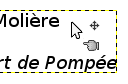
\includegraphics[angle=0,width=.4\textwidth]{./images/image02/TexteCurseurBougePas}
\end{minipage}\hfill%
\begin{minipage}[c]{.46\textwidth}
\centering%
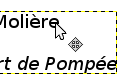
\includegraphics[angle=0,width=.4\textwidth]{./images/image02/TexteCurseurBouge}
\end{minipage}\\[12pt]
\begin{minipage}[c]{.46\textwidth}
{\small \emph{Avec un curseur de cette forme, c'est le calque qui se déplace.}}
\end{minipage}\hfill%
\begin{minipage}[c]{.46\textwidth}
{\small \emph{Avec un curseur de cette forme, c'est le texte qui se déplace.}}
\end{minipage}

\vspace{1em}

\textbf{Remarque :} on peut déplacer le texte directement sans chercher la bonne position en se plaçant sur le texte et en maintenant la touche \texttt{Shift} enfoncée.



\subsection{Appliquer un filtre sur une portion de l'image}\index{Gimp!Appliquer un filtre}\index{Appliquer un filtre (Gimp)}\label{Gimp2AppliquerFiltre}

Nous allons flouter un visage pour montrer l'usage d'un filtre sur une portion de l'image.

Pour cela, il faut sélectionner la partie souhaitée à l'aide d'un des outils de sélection. On peut sélectionner une zone rectangulaire 
\includegraphics[width=.6cm]{./images/image02/iconeSelecRectangle}, une zone ovale 
\includegraphics[width=.6cm]{./images/image02/iconeSelecOvale} ou sélectionner une zone <<\,à main levée\,>> 
\includegraphics[width=.6cm]{./images/image02/iconeSelecLasso}.

\vspace{6pt}

Attention, si un texte a été ajouté auparavant sur l'image, il faut se repositionner sur le calque correspondant à l'image (se reporter si nécessaire à la section \vref{Gimp2Calques}). 

\vspace{6pt}

Sur la figure ci-dessous, le visage a été sélectionné à l'aide de l'outil de sélection ovale.

\uneimageici{./images/image02/FiltrePixel1}{.55\textwidth}

Une fois la zone sélectionnée, dans le menu \texttt{Filtres}, choisir \texttt{Flou}, puis \texttt{Pixéliser...}   

\uneimageici{./images/image02/FiltrePixel2}{.6\textwidth}

Dans la boîte de dialogue qui s'ouvre alors (figure à gauche ci-dessous), modifier les paramètres afin d'obtenir le résultat souhaité puis cliquer sur le bouton \texttt{OK}. Le résultat obtenu est montré sur la figure de droite ci-dessous.

\deuximagesici{./images/image02/FiltrePixel3}{.6\textwidth}%
              {./images/image02/FiltrePixel4}{.6\textwidth}




\subsection{Convertir une image en noir et blanc}\index{Gimp!Convertir en niveaux de gris}\index{Convertir en niveaux de gris (Gimp)}\label{Gimp2ConvertirNoirBlanc}

 Pour convertir une image couleur en noir et blanc (le terme exact est en \emph{niveaux de gris}), il faut, dans le menu \texttt{Image}, choisir \texttt{Mode} puis \texttt{Niveaux de gris}. L'image est immédiatement convertie. Remarque : on peut également faire directement un clic droit sur l'image (comme montré sur la figure ci-dessous), puis choisir \texttt{Image}, \texttt{Mode} et \texttt{Niveaux de gris}.

\deuximagesGPici{./images/image02/NoirBlanc1}{\textwidth}%
              {./images/image02/NoirBlanc2}{.6\textwidth}




\subsection{Travailler avec les calques}\label{Gimp2Calques}\index{Calques}\index{Gimp!Calques}

Dans Gimp il est possible de travailler avec des \emph{calques} qui correspondent à des couches successives que l'on ajoute sur l'image de base. L'image finale correspond alors à la superposition de tous les calques. Toute la gestion des calques se passe dans la fenêtre des calques.

\vspace{6pt}

Observez l'exemple ci-dessous : l'image de droite est composée de trois calques, représentés séparément à gauche.

\vspace{12pt}

\begin{minipage}[c]{.22\textwidth}
\centering%
\fbox{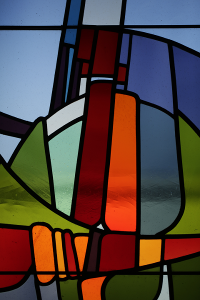
\includegraphics[angle=0,width=.7\textwidth]{./images/image02/exempleCalquesVitraux}}
\end{minipage}\hfill%
\begin{minipage}[c]{.22\textwidth}
\centering%
\fbox{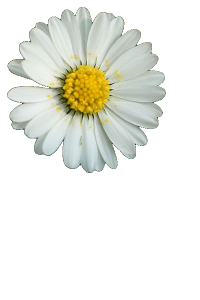
\includegraphics[angle=0,width=.7\textwidth]{./images/image02/exempleCalquesFleur}}
\end{minipage}\hfill%
\begin{minipage}[c]{.22\textwidth}
\centering%
\fbox{
\includegraphics[angle=0,width=.7\textwidth]{./images/image02/exempleCalquesCinq}}
\end{minipage}\hfill%
\begin{minipage}[c]{.22\textwidth}
\centering%
\fbox{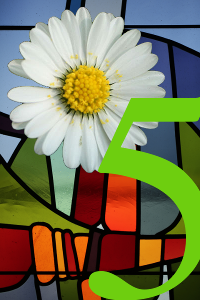
\includegraphics[angle=0,width=.7\textwidth]{./images/image02/exempleCalques}}
\end{minipage}\\[12pt]
\begin{minipage}[c]{.22\textwidth}
\centering {\footnotesize Calque 1 : le fond.}
\end{minipage}\hfill%
\begin{minipage}[c]{.22\textwidth}
\centering {\footnotesize Calque 2 : la fleur.}
\end{minipage}\hfill%
\begin{minipage}[c]{.22\textwidth}
\centering {\footnotesize Calque 3 : le 5.}
\end{minipage}\hfill%
\begin{minipage}[c]{.22\textwidth}
\centering {\footnotesize L'image finale.}
\end{minipage}


\vspace{12pt}

La figure ci-dessous montre la fenêtre des calques correspondant à l'image ci-dessus : on y retrouve bien les trois calques correspondant à chacune des couches. Attention, l'ordre des calques est très important : le calque le plus haut de la pile cache les autres (ici la fleur est au-dessus du fond et le 5 est au-dessus de la fleur et du fond).

\uneimageici{./images/image02/CalqueFenetre}{.4\textwidth}





\subsubsection{Ajouter un calque}\label{Gimp2CalquesAjouter}\index{Calques : ajouter}\index{Gimp!Ajouter un calque}

Pour ajouter un calque, il faut se rendre dans la fenêtre des calques et cliquer sur l'icône 
\includegraphics[width=.4cm]{./images/image02/CalqueAjouter} (figure ci-dessous à gauche). Une boîte de dialogue s'ouvre alors (figure ci-dessous au centre) : elle permet de choisir le nom du calque (que l'on peut modifier par la suite en double-cliquant sur celui-ci) et le type de remplissage (choisir \texttt{Transparence}). Le nouveau calque apparaît alors dans la fenêtre des calques (figure ci-dessous à droite).

\vspace{12pt}

\begin{minipage}[c]{.32\textwidth}
\centering%
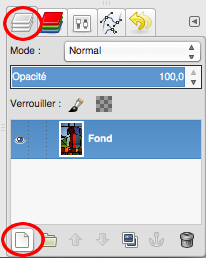
\includegraphics[angle=0,width=.85\textwidth]{./images/image02/GimpCalqueAjouter1}
\end{minipage}\hfill%
\begin{minipage}[c]{.32\textwidth}
\centering%
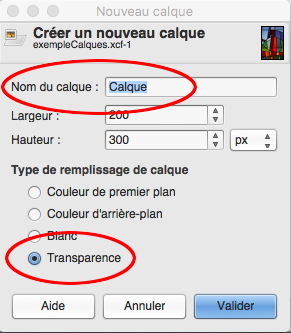
\includegraphics[angle=0,width=.85\textwidth]{./images/image02/GimpCalqueAjouter2}
\end{minipage}\hfill%
\begin{minipage}[c]{.32\textwidth}
\centering%
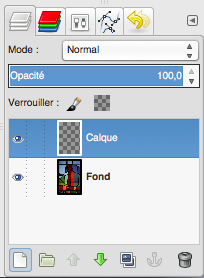
\includegraphics[angle=0,width=.85\textwidth]{./images/image02/GimpCalqueAjouter3}
\end{minipage}

\vspace{12pt}

Remarque importante : le \emph{calque actif}\index{Calques : changer de calque actif}\index{Gimp!Changer de calque actif}, c'est-à-dire le calque sur lequel on est en train de travailler, apparaît coloré dans la fenêtre des calques.


\subsubsection{Modifier l'opacité d'un calque}\label{Gimp2CalquesOpacite}\index{Calques : modifier l'opacité}\index{Gimp!Modifier l'opacité d'un calque} 

\emph{Modifier l'opacité} d'un calque signifie le rendre plus ou moins transparent afin que l'on puisse <<\,voir à travers\,>>.

Pour modifier l'opacité d'un calque, il suffit de le rendre actif en cliquant dessus dans la fenêtre des calques, puis de modifier la valeur de l'opacité à l'aide du curseur \texttt{Opacité} 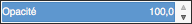
\includegraphics[width=3.5cm]{./images/image02/BarreOpacite}. Si le calque est opaque à 100\,\%\ alors on ne voit pas les calques situés au-dessous. Si le calque a une opacité de 0\,\%\, alors il n'est plus visible. Pour rendre invisible un calque, il est également possible de cliquer sur l'œil 
\includegraphics[width=.6cm]{./images/image02/iconeOeil} dans la fenêtre des calques.

Sur la figure ci-dessous, le calque contenant la fleur a une opacité de 70\,\% : on voit donc le fond par transparence à travers la fleur.  

\uneimageici{./images/image02/GimpCalqueOpacite2}{.55\textwidth}



\subsubsection{Modifier la pile des calques}\label{Gimp2CalquesOrdonner}\index{Calques : modifier la pile des calques}\index{Gimp!Modifier la pile des calques}

Tous les calques sont empilés les uns sur les autres. Le calque le plus bas dans la pile est recouvert par tous les autres. Il est parfois nécessaire de modifier la position d'un calque dans la pile des calques. Pour cela, deux solutions sont possibles :
\begin{itemize}
\item déplacer simplement le calque dans la fenêtre des calques à l'aide de la souris en effectuant un glisser-déposer ;
\item utiliser les boutons de déplacement du calque actif 
\includegraphics[width=1cm]{./images/image02/CalqueOrdonner} situés en bas de la fenêtre des calques.
\end{itemize}




\subsubsection{Déplacer un calque}\label{Gimp2CalquesDeplacer}\index{Calques : déplacer le calque}\index{Gimp!Déplacer un calque} 

À l'aide de l'outil de déplacement 
\includegraphics[width=.4cm]{./images/image02/iconeDeplacement} disponible dans la palette d'outils (figure ci-dessous à gauche), il est possible de déplacer le calque actif. Sur la figure à droite ci-dessous, le calque contenant la fleur (dont le contour est visible, en pointillés noir et jaune) est déplacé à l'aide de la souris. 

\deuximagesPGici{./images/image02/GimpCalqueDeplacer1}{.5\textwidth}%
              {./images/image02/GimpCalqueDeplacer2}{.9\textwidth}






\subsection{Réaliser une copie d'écran}\label{CaptureEcran2}\index{Capture d'écran}\index{Gimp!Capture d'écran}

Il est parfois nécessaire de copier le contenu de l'écran sous forme d'image pour pouvoir l'utiliser dans un document ou une présentation.

\vspace{12pt}

Pour réaliser une copie d'écran :

\begin{enumerate}
\item Capturer l'écran en utilisant un des raccourcis clavier suivant :
        \begin{itemize}
        \item \texttt{Ctrl + Maj + Cmd + 3} pour copier la totalité de l'écran,\index{Raccourci Clavier! Ctrl + Maj + Cmd + 3, copier tout l'écran}
        \item \texttt{Ctrl + Maj + Cmd + 4} pour copier une partie de l'écran (à sélectionner à la souris) ;\index{Raccourci Clavier! Ctrl + Maj + Cmd + 4, copier une partie de l'écran}
        \end{itemize} 

\uneimageici{./images/generales/clavierCapEcran}{.6\textwidth}

\item Coller l'image dans un nouveau document sous \emph{Gimp} : 
\end{enumerate}

\uneimageici{./images/image02/GimpCollerCommeImage}{.6\textwidth}

On peut alors retravailler l'image comme vous l'avez appris dans cette fiche sur \emph{Gimp}. 




\newpage

%
%
%  S  É  A  N  C  E     I
%
%


\section{Séance 1 : un haïku écrit sur une image}\label{ficheImage5e1}

\boiteEnonceLarge{Le but de cette séance est d'écrire un haïku sur une image, comme le montre l'exemple ci-dessous. Pour parvenir à ce résultat, vous devrez utiliser les outils présentés en début de chapitre (voir section \vref{Image5eOutils}).\\[4pt]
%
Un \emph{haïku} est un poème très court dont le but est de dire et de célébrer l'évanescence des choses\footnote{D'après la définition donnée sur la page Wikipedia du haïku.}. Ce type de poème a été inventé au Japon au XVIIe siècle.
%
\begin{enumerate}
\item Écrire un poème de type haïku de votre choix.
\item Se rendre sur le site d'images librement utilisables \url{https://www.pexels.com} et choisir une image pour illustrer votre poème. La télécharger en taille \emph{medium} (l'enregistrer sur le \emph{Bureau} de l'ordinateur pour la retrouver facilement). Ce site est une bibliothèque d'images sous \emph{licence libre} qu'il est donc possible d'utiliser et de modifier librement\footnote{Pour obtenir davantage d'informations sur les licences libres, se rendre sur le site de \emph{Creative Commons} \url{https://creativecommons.fr/}.}.
\item Ouvrir l'image à l'aide du logiciel Gimp. Si une boîte de dialogue s'ouvre pour vous proposez de convertir le profil de couleur de l'image, cliquer sur \texttt{Convertir}.
\item Si nécessaire, recadrer l'image ou convertir l'image en niveaux de gris.
\item Sélectionner une zone de l'image (là où vous allez écrire le poème) et ajouter un flou gaussien (menu \texttt{Filtre}, choisir \texttt{Flou} puis \texttt{Flou gaussien}).   
\item La zone étant toujours sélectionnée, augmenter la luminosité afin d'éclaircir l'image à cet endroit (menu \texttt{Couleurs}, choisir \texttt{Luminosité-Contraste}). 
\item Ajouter alors le texte du poème et régler la police de caractères, la couleur et la taille des caractères. Positionner le texte à l'endroit de votre choix.
\item Pour aller plus loin (facultatif), ajouter un cadre autour de l'image.
\item Une fois le travail terminé, exporter l'image au format PNG (le fichier doit être nommé à partir de votre nom : \texttt{Nom-Prénom-date.png}) et le rendre sur la plateforme Moodle à l'endroit indiqué par votre enseignant.
\end{enumerate}
}% fin de l'énoncé


\begin{minipage}[c]{.48\textwidth}
L'objectif est d'obtenir une image comme par exemple celle montrée ci-contre (haïku écrit par \emph{Bash\={o} Matsuo}, un des quatre maîtres classiques de la discipline).
\end{minipage}\hfill%
\begin{minipage}[c]{.48\textwidth}
\centering%
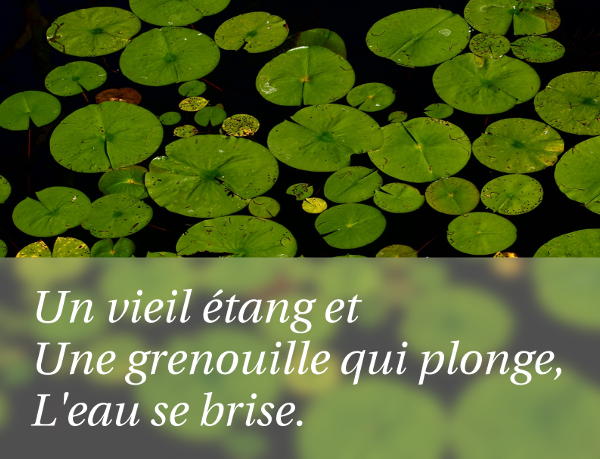
\includegraphics[angle=0,width=.8\textwidth]{./images/image02/haiku}
\end{minipage}





%
%
%  S  É  A  N  C  E     II
%
%


\section{Séance 2 : superposition d'images}\label{ficheImage5e2}


\boiteEnonceLarge{Le but de cette séance est de superposer des images et d'utiliser les réglages d'opacité des calques afin d'en obtenir une nouvelle, comme le montre l'exemple ci-dessous. Pour parvenir à ce résultat, vous devrez utiliser les outils présentés en début de chapitre (voir section \vref{Image5eOutils}).

%
\begin{enumerate}
\item Récupérer trois images de base sur la page Moodle de votre cours.
\item Ouvrir une de ces images sous Gimp.
\item Créer deux nouveaux calques (leur donner un nom explicite) et y copier les deux autres images : vous devez alors avoir sous Gimp une image composée de trois calques qui contiennent chacun une image fournie par l'enseignant.
\item Choisir l'ordre des calques en utilisant les flèches 
\includegraphics[width=1cm]{./images/image02/CalqueOrdonner} situées en bas de la fenêtre des calques, afin que l'image utilisée comme arrière-plan apparaisse tout en bas de la pile de calque. Faire de même pour les deux autres images (les positionner au bon endroit). 
\item Régler l'opacité des deux calques du haut à 50\,\%\ afin de voir par transparence les trois images.  
\item À l'aide de l'outil de déplacement des calques 
\includegraphics[width=.4cm]{./images/image02/iconeDeplacement}, positionner chacune des images à l'endroit souhaité. Utiliser si nécessaire l'œil 
\includegraphics[width=.6cm]{./images/image02/iconeOeil} qui permet d'afficher ou non un calque.
\item Une fois le positionnement effectué, terminer de régler l'opacité des calques pour obtenir le résultat désiré.
\item Ajouter prénom et nom à l'aide de l'outil d'ajout de texte et effectuer sa mise en forme.
\item Pour aller plus loin (facultatif), ajouter un cadre autour de l'image.
\item Une fois le travail terminé, exporter l'image au format PNG (le fichier doit être nommé à partir de votre nom : \texttt{Nom-Prénom-date.png}) et le rendre sur la plateforme Moodle à l'endroit indiqué par votre enseignant.
\end{enumerate}
}% fin de l'énoncé


L'objectif est d'obtenir une image comme par exemple celle montrée ci-dessous (à gauche les trois images de base utilisées et à droite l'image finale obtenue).

\vspace{12pt}

\begin{minipage}[c]{.38\textwidth}
\begin{center}
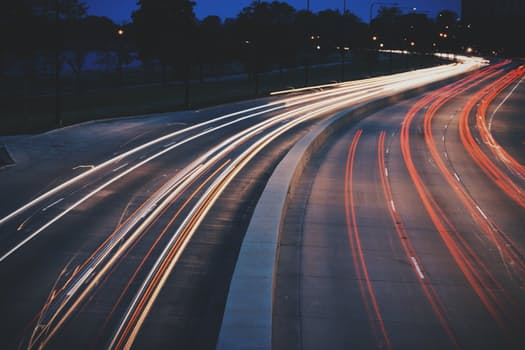
\includegraphics[angle=0,width=.4\textwidth]{./sources/image02/seanceArts/01_Road}

\vspace{4pt}

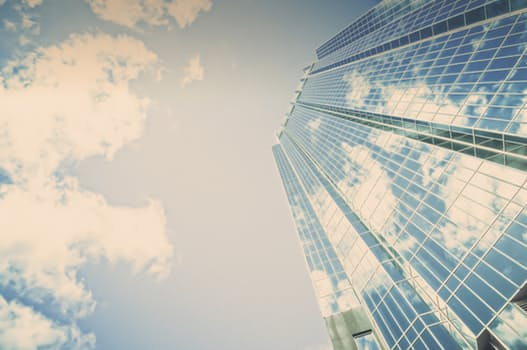
\includegraphics[angle=0,width=.4\textwidth]{./sources/image02/seanceArts/02_Tower}

\vspace{4pt}

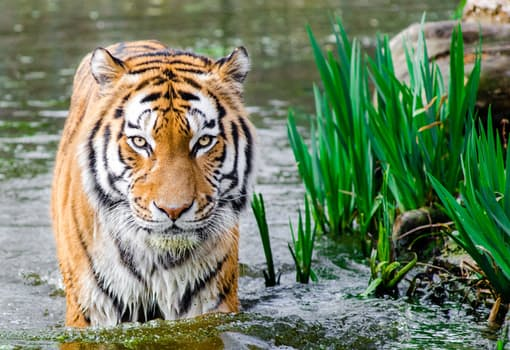
\includegraphics[angle=0,width=.4\textwidth]{./sources/image02/seanceArts/03_Tiger}
\end{center}
\end{minipage}\hfill%
\begin{minipage}[c]{.6\textwidth}
\centering%
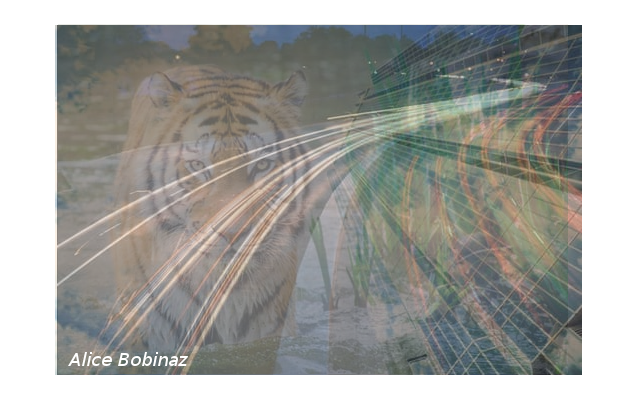
\includegraphics[angle=0,width=.85\textwidth]{./sources/image02/seanceArts/seanceArts5e}
\end{minipage}

